% !TeX root = ../../main.tex
\subsection{工具总体结构设计}
\label{kebianjingguaguan}
GGQ95型可变径套管刮管器（图纸型号BJG700000A，7\inch 可变径刮壁器）是一种可通过 7\inch 套管、仅在 9-5/8\inch 套管内张开的液压可变径刮管工具：其刮刀收回外径为 136\,mm、工具本体最大外径为 139.5\,mm，均小于 7\inch 套管的内径（随磅级约为 145$\sim$166\,mm），因此下井及通过 7\inch 套管时刮刀始终收回、与井壁不接触，7\inch 套管的刮管由同趟管柱中位于本工具下方的常规 7\inch 刮管器完成；待管柱上提至 9-5/8\inch 套管井段并投球憋压激活后，刮刀方可张开（自由张开外径 229\,mm 以上，实际受 9-5/8\inch 套管内径约束贴壁），清除 9-5/8\inch 套管内壁上的残余水泥、泥块、轧制过程中产生的毛刺与鳞片、管内防砂射孔时镶在管壁上的射孔弹、生产井套管上的铁锈与水垢以及硬石蜡等影响正常施工作业的杂物；本工具与常规 7\inch 刮管器组合，实现"一趟钻完成 7\inch 与 9-5/8\inch 套管刮管"。其结构如图~\ref{fig:variable_scrapter_structure}所示，可变径套管刮削器由上接头、旋转连杆座、连杆、刮刀、芯轴、复位总成、工作活塞、工作弹簧、下接头、节流喷嘴、中间外筒、中间芯轴、激活球座、钢球以及标准件、密封件等零件组成（图纸BJG700000A总装图：上接头BJG700001A、上活动连杆座BJG700002A、连杆BJG700003A、刮刀芯轴BJG700004A、活动座铰链销BJG700005A、59BPF刮刀BJG700006A、刮刀铰链销BJG700007A、下活动连杆座BJG700008A、连杆座连接筒BJG700009A～中间筒体BJG700013A、心轴连接筒BJG700014A、球座BJG700015A、丝堵BJG700016A、密封堵BJG700017A、复位弹簧BJG700018A、工作弹簧BJG700019A、下接头BJG700020A、支撑弹片BJG700021A、弹片压块BJG700022A、$\phi 25$节流喷嘴BJG700023A）。刮刀采用两组 5 瓣圆周错位排布，覆盖 9-5/8\inch 套管内径圆周 360° 方向。

该工具的工作原理为：下井及通过 7\inch 套管时，球座由圆周 $4\times\phi 4.80$ 剪钉定位于上位，将活塞腔与工具水眼流道隔断，刮刀由复位弹簧保持在收回位（收回外径 136\,mm），工具处于\textbf{收回待命状态}，此时可正常循环、旋转并传递扭矩与提拉、下放载荷，球未落座时泵压再高刮刀也不会张开；投球后钢球坐封球座、憋压剪断剪钉，球座下移并建立活塞腔与工具水眼流道，水眼内的液压力经工具底部节流喷嘴形成的工作压差推动工作活塞并迫使工作弹簧上行，在连杆机构的作用下刮刀张开、贴紧 9-5/8\inch 套管内壁；随后上提、下放管柱即可实现刮刀对套管内壁的刮削清洁，停泵后节流压差消失、刮刀由复位弹簧收回。工具激活为一次性、不可逆过程（图纸明细栏中不设复位球），因此 7\inch 套管的全部作业必须在投球激活之前完成。工具的上下接头分别连接管柱，并通过芯轴连接，可传递扭矩和提拉、下放载荷；旋转连杆座可迫使整组刮刀绕工具自由旋转，当套管内壁变形或通过性较差时，刮刀可绕工具旋转错位通过。该工具的三个工作状态见表~\ref{tab:ggq95_states}，技术参数见表~\ref{tab:ggq95}。

\begin{table}[htbp]
    \centering
    \caption{可变径刮管器工作状态}
    \label{tab:ggq95_states}
    \footnotesize
    \setlength{\tabcolsep}{4pt}
    \renewcommand{\arraystretch}{1.3}
    \begin{tabular}{p{2.4cm}p{2.6cm}p{2.2cm}p{2.6cm}p{3.4cm}}
        \toprule
        工作状态 & 球座位置 & 剪钉与活塞腔 & 刮刀外径 & 可进行的作业 \\
        \midrule
        收回待命（投球前） & 上位，隔断活塞腔与水眼流道 & 剪钉完好、完好隔断 & 136\,mm（本体 139.5\,mm） & 循环、旋转、传递扭矩、通过 7\inch 套管，由下部常规 7\inch 刮管器完成 7\inch 段刮管及其它作业 \\
        激活（投球憋压） & 剪钉剪断、球座下移，不可逆 & 流道建立、活塞腔连通 & 由 136\,mm 开始张开 & 出现"泵压先升后突降"的激活特征 \\
        张开刮削（激活后循环） & 下位（永久） & 连通，节流工作压差 $\le 4$\,MPa & 张开贴壁（自由张开 229\,mm 以上） & 上提、下放刮削 9-5/8\inch 套管 \\
        停泵（激活后） & 下位（永久） & 连通但无压差 & 复位弹簧收回至 136\,mm & 起钻，通过内径较小的井段 \\
        \bottomrule
    \end{tabular}
\end{table}

\begin{figure}[htbp]
	\centering
	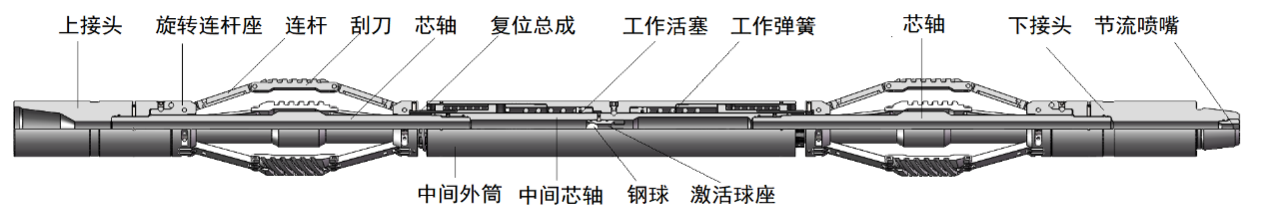
\includegraphics[width=1.\textwidth]{figure/chapter3/part5/variable-scrapter-structure.png}
	\caption{可变径刮管器结构示意图}
	\label{fig:variable_scrapter_structure}
\end{figure}

\begin{table}[htbp]
    \centering
    \caption{GGQ95型可变径套管刮管器技术参数}
    \label{tab:ggq95}
    \renewcommand{\arraystretch}{1.2} % 适当增加行高，提升阅读体验
    \small % 调整整体字号，适应表格宽度
    \begin{tabular}{ccccccc}
        \toprule
        型号 & \begin{tabular}[c]{@{}c@{}}本体最大外径\\(mm)\end{tabular} & \begin{tabular}[c]{@{}c@{}}刮刀收回最小外径\\(mm)\end{tabular} & \begin{tabular}[c]{@{}c@{}}刮刀最大外径\\(mm)\end{tabular} & \begin{tabular}[c]{@{}c@{}}水眼\\(mm)\end{tabular} & \begin{tabular}[c]{@{}c@{}}总长\\(mm)\end{tabular} & \begin{tabular}[c]{@{}c@{}}接头扣\\(API)\end{tabular} \\
        \midrule
        GGQ95 & 139.50 & 136 & 229+ & 38.1 & 2959.61 & NC38 \\
        \bottomrule
    \end{tabular}
\end{table}

注：本体最大外径按图纸BJG700000A总装图标注的$\phi 139.50$取139.50\,mm；总长按总装图标注的$2959.61\pm 2.50\,\text{mm}$取2959.61\,mm；水眼为工具最小过流内径，取图纸BJG700004A刮刀芯轴内孔$\phi 38.10$；接头扣按总装图NC38（API 7-2）标注。


\subsection[可变径刮管工具设计计算与校核]{可变径刮管工具设计计算与校核\protect\footnote{合同条款：5.2.1.3井筒高效清洁关键技术配套工具设计——（4）可变径刮管工具：抗拉$>=100\mathrm{T}$，抗扭$>17\,\mathrm{kN}\cdot\mathrm{m}$}}


\subsubsection{主要受力件的螺纹强度校核}

9-5/8\inch 可变径刮壁器的主要受力件为刮刀芯轴，其主要受力螺纹为 $\mathrm{Tr}\,65 \times 4-8e$，危险截面即位于该螺纹的根部。

螺纹牙的剪切强度按下式计算：
\begin{equation}
	\begin{aligned}
	    F_{\max} &= [\tau] \cdot k_z \cdot \pi \cdot d_1 \cdot b \cdot z \cdot 10^{-3} \\
	    [\tau] &= \frac{\sigma_s}{n}
	\end{aligned}
	\end{equation}
	
式中，$F_{\max}$---工具最大拉力，kN；

$[\tau]$---螺纹牙的许用剪切强度，MPa；

$k_z$---螺纹各圈的载荷不均系数，根据《机械设计手册》螺纹连接（紧固件连接）部分中螺纹牙的剪切强度计算及各圈螺纹载荷分配的规定\cite{ref26}，取 $k_z = 0.56$；

$d_1$---螺纹底径，按图纸BJG700004A刮刀芯轴左端标注的 $\mathrm{Tr}\,68\times4-8e$ 螺纹小径并按牙型高度换算取 $d_1 = 62\,\text{mm}$；

$b$---螺纹牙根宽度，mm；按GB/T 5796规定的梯形螺纹牙型，由螺距$p=4\,\text{mm}$与牙型高度计算得 $b = 2.6\,\text{mm}$；

$z$---旋合圈数，由图纸BJG700004A刮刀芯轴左端旋合长度$94\,\text{mm}$除以螺距$4\,\text{mm}$得到，$z = 23.5$；

$\sigma_s$---材料最小屈服强度，刮刀芯轴材料为 4330V（屈服强度 $1068\,\mathrm{MPa}$），取 1068 MPa；

$n$---安全系数，根据《机械设计手册》螺纹连接部分中螺纹牙强度校核的安全系数取值规定\cite{ref26}，取 $n = 2.5$。

将 $\mathrm{Tr}\,65 \times 4-8e$ 螺纹的相关参数代入，计算得：
\begin{equation}
    \begin{aligned}
    F_{\max} &= [\tau] \cdot k_z \cdot \pi \cdot d_1 \cdot b \cdot z \cdot 10^{-3} \\
             &= 427.2 \times 0.56 \times 3.14 \times 62 \times 2.6 \times 23.5 \times 10^{-3} \\
             &= 2845.65\,\mathrm{kN} \\
             &> 1000\,\mathrm{kN}
    \end{aligned}
\end{equation}
计算结果表明，螺纹牙的剪切强度满足设计要求。


\subsubsection{主要受力件的零件抗拉强度校核}

9-5/8\inch 可变径刮壁器的主要受力件为刮刀芯轴和芯轴连接筒，两者的抗拉危险截面分别为刮刀芯轴小螺纹 $\mathrm{Tr}\,65 \times 4-8e$ 螺纹根部和芯轴连接筒内螺纹 $\mathrm{Tr}\,65 \times 4-8H$ 螺纹根部。

抗拉强度按下式计算：
\begin{equation}
    F_{\max} = \frac{\pi \cdot (D^2 - d^2) \cdot \sigma_s}{4 \cdot n} \times 10^{-3}
\end{equation}
式中，$F_{\max}$---工具最大拉力，kN；

$D$---危险截面外径，mm；各受力件取值如下：

\quad 刮刀芯轴：按图纸BJG700004A标注的左端牙槽根外圆 $\phi 58\,{-0.03}/{-0.048}$ 与螺纹底径取 $D = 62\,\text{mm}$；

\quad 芯轴连接筒：按图纸BJG700014A标注的外圆 $\phi 80\,{-0.03}/{-0.06}$ 取 $D = 80\,\text{mm}$；

$d$---危险截面内径，mm；各受力件取值如下：

\quad 刮刀芯轴：按图纸BJG700004A标注的内孔 $\phi 38.10$（即工具水眼）取 $d = 38.1\,\text{mm}$；

\quad 芯轴连接筒：按图纸BJG700014A标注的内螺纹 $\mathrm{Tr}\,65\times4-8H$ 小径 $\phi 62.20\,{+0.07}/0$ 取 $d = 62.2\,\text{mm}$（原稿取66\,mm与图纸标注不符，已更正）；

$\sigma_s$---材料最小屈服强度；刮刀芯轴与芯轴连接筒材料均为 4330V（屈服强度 $1068\,\mathrm{MPa}$），取 1068 MPa；

$n$---安全系数，取 $n = 1.5$。

（1）刮刀芯轴危险截面最大抗拉计算
\begin{equation}
    \begin{aligned}
    F_{\max} &= \frac{\pi \cdot (D^2 - d^2) \cdot \sigma_s}{4 \cdot n} \times 10^{-3}
             = \frac{3.14 \times (62^2 - 38.1^2) \times 1068}{4 \times 1.5} \times 10^{-3} \\
             &= 1337.15\,\mathrm{kN} > 1000\,\mathrm{kN}
    \end{aligned}
\end{equation}
满足设计要求。

（2）芯轴连接筒危险截面最大抗拉计算
\begin{equation}
    \begin{aligned}
    F_{\max} &= \frac{\pi \cdot (D^2 - d^2) \cdot \sigma_s}{4 \cdot n} \times 10^{-3}
             = \frac{3.14 \times (80^2 - 66^2) \times 1068}{4 \times 1.5} \times 10^{-3} \\
             &= 1142.43\,\mathrm{kN} > 1000\,\mathrm{kN}
    \end{aligned}
\end{equation}
满足设计要求。

需要说明的是，芯轴连接筒的危险截面应取内螺纹 $\mathrm{Tr}\,65\times4-8H$ 根部（小径 $\phi 62.20$，见图BJG700014A），此时
\begin{equation}
    \begin{aligned}
    F_{\max} &= \frac{3.14 \times (80^2 - 62.2^2) \times 1068}{4 \times 1.5} \times 10^{-3}
             = 1414.72\,\mathrm{kN} > 1000\,\mathrm{kN}
    \end{aligned}
\end{equation}
亦满足设计要求。按图纸BJG700014A的技术要求，该件材料为 4330V（屈服强度$\ge 1068$\,MPa，抗拉强度$\ge 1180$\,MPa，硬度341$\sim$401\,HB），与刮刀芯轴同一材料等级，故上述两个截面的许用拉力分别为 $1142.43\,\mathrm{kN}$（$\phi 80/\phi 66$）与 $1414.72\,\mathrm{kN}$（$\phi 80/\phi 62.2$）；在 $1000\,\mathrm{kN}$ 轴向拉力作用下，两截面的名义拉应力分别为 $623.2\,\mathrm{MPa}$ 与 $503.3\,\mathrm{MPa}$，对应 $1068\,\mathrm{MPa}$ 屈服强度的安全系数分别为 $1.71$ 与 $2.12$，均大于设计要求的 1.5。


\subsubsection{主要受力件的零件抗扭强度校核}

9-5/8\inch 可变径刮壁器的主要受力件为刮刀芯轴和芯轴连接筒，其抗扭危险截面与抗拉校核相同，分别位于刮刀芯轴小螺纹 $\mathrm{Tr}\,65 \times 4-8e$ 螺纹根部和芯轴连接筒内螺纹 $\mathrm{Tr}\,65 \times 4-8H$ 螺纹根部。

抗扭强度按下式计算：
\begin{align}
    \tau &= \frac{16 \cdot D \cdot T_{\max}}{\pi \cdot (D^4 - d^4)} \times 10^{6} \\
    T_{\max} &= \frac{[\tau] \cdot \pi \cdot (D^4 - d^4)}{16 \cdot D} \times 10^{-6} \\
    [\tau] &= n \cdot \sigma_s = 0.66 \times 1068\,\mathrm{MPa} = 704.88\,\mathrm{MPa}
\end{align}
式中，$T_{\max}$---工具最大扭矩，$\mathrm{kN}\cdot\mathrm{m}$；

$\tau$---危险截面的切应力，MPa；

$[\tau]$---材料许用切应力，MPa；

$\sigma_s$---材料屈服强度，取 1068 MPa；

$D$---危险截面外径，mm；各受力件取值与抗拉校核相同（刮刀芯轴 $D = 62\,\text{mm}$、芯轴连接筒 $D = 80\,\text{mm}$）；

$d$---危险截面内径，mm；各受力件取值与抗拉校核相同（刮刀芯轴 $d = 38.1\,\text{mm}$、芯轴连接筒 $d = 66\,\text{mm}$）；

$n$---许用切应力与许用拉应力之比，根据《机械设计手册》零件强度校核中许用应力折减系数的取值规定\cite{ref26}，取 $n = 0.66$（其理论依据为第四强度理论，纯剪切时 $\tau_s = \sigma_s/\sqrt{3} \approx 0.577\sigma_s$，工程上取 $0.66$ 作为折减系数）。

（1）刮刀芯轴危险截面最大抗扭计算
\begin{equation}
    \begin{aligned}
    T_{\max} &= \frac{[\tau] \cdot \pi \cdot (D^4 - d^4)}{16 \cdot D} \times 10^{-6}
             = \frac{704.88 \times 3.14 \times (62^4 - 38.1^4)}{16 \times 62} \times 10^{-6} \\
             &= 28.27\,\mathrm{kN}\cdot\mathrm{m} > 17\,\mathrm{kN}\cdot\mathrm{m}
\end{aligned}
\end{equation}
满足设计要求。

（2）芯轴连接筒危险截面最大抗扭计算
\begin{equation}
    \begin{aligned}
    T_{\max} &= \frac{[\tau] \cdot \pi \cdot (D^4 - d^4)}{16 \cdot D} \times 10^{-6}
             = \frac{704.88 \times 3.14 \times (80^4 - 66^4)}{16 \times 80} \times 10^{-6} \\
             &= 38.02\,\mathrm{kN}\cdot\mathrm{m} > 17\,\mathrm{kN}\cdot\mathrm{m}
\end{aligned}
\end{equation}
满足设计要求。


\subsubsection{球座剪钉剪切力与节流泵压计算}

9-5/8\inch 可变径刮壁器需要投球后憋压将球座剪钉剪断，迫使球座下移建立压力通道才能开始工作，因此剪钉的剪断力和投球后球座处的憋压压力是激活工具的重要参数。

刮壁器的球座圆周设计 4 组剪钉参与剪切（图纸BJG700015A球座标注 $4\times 4.80\,{+0.20}/0$ 剪钉孔），剪钉选用 45 号非调质料制作，则工具激活所需的推力为：
\begin{equation}
    \begin{aligned}
        F_s \ge [\tau] \cdot A = 0.6 \times [\sigma] \times 4 \times (\pi \cdot R^2) &= 0.6 \times 450 \times 4 \times 3.14 \times 2.4^2 \\
        &= 19534.4\,\mathrm{N}
    \end{aligned}
\end{equation}
式中，$F_s$---工具激活所需的最小推力，N；

$[\tau]$---材料许用剪应力，塑性材料取 $0.6[\sigma]$、脆性材料取 $0.8[\sigma]$；45 号钢为塑性材料，故按 $0.6[\sigma]$ 取值，即 $0.6\times450 = 270\,\mathrm{MPa}$；

$[\sigma]$---材料许用拉应力，按45号钢的屈服强度取 $450\,\mathrm{MPa}$；

$A$---参与剪切的剪钉总剪切面积，$\mathrm{mm}^2$；$A = n_s \cdot \pi R^2$，$n_s$ 为剪钉数量，按图纸取 $n_s = 4$；

$R$---单个剪钉的半径，mm；按图纸BJG700015A标注的剪钉孔径取 $R = 2.4\,\mathrm{mm}$。

刮壁器投入钢球后球座流道被堵塞，井口泵压直接作用在球座上，根据上述计算所得的最小推力 $F_s$，可计算出激活工具所需的最小泵压 $P_0$：
\begin{equation}
    P_0 \ge \frac{F_s}{A_q} = \frac{F_s}{\pi \cdot \left(\frac{d}{2}\right)^2} = \frac{19534.4}{3.14 \times \left(\frac{40.08}{2}\right)^2} = 15.48\,\mathrm{MPa}
\end{equation}
式中，$P_0$---激活工具所需的最小泵压，MPa；

$A_q$---球座承压面积，$\mathrm{mm}^2$；

$d$---球座承压面直径，mm；按图纸BJG700015A球座标注的锥面大径取 $d = 40.08\,\text{mm}$。原稿取工具球座外径45\,mm，使承压面积偏大、泵压偏小，已按图纸更正。

计算表明，当泵压不小于 $15.48\,\mathrm{MPa}$ 时，工具可以被激活。若按脆性材料系数 $0.8[\sigma]$ 偏安全计算，则 $F_s = 26045.9\,\mathrm{N}$，对应最小泵压为 $20.65\,\mathrm{MPa}$，两种取值下激活泵压均在常规作业泵压范围内。


\subsubsection{节流喷嘴的尺寸和节流压力关系}

刮壁器激活后流道建立，工具底部的节流喷嘴形成的节流压差为工具提供工作压力 $\Delta P \le 4\,\mathrm{MPa}$，故需要计算节流喷嘴的尺寸与节流压力的关系。

由公式：
\begin{equation}
    \Delta P \le \frac{827 \cdot \rho \cdot Q^2}{C^2 \cdot d_e^4}
\end{equation}

推算喷嘴最小直径为：
\begin{equation}
    d_e \ge \sqrt[4]{\frac{827 \cdot \rho \cdot Q^2}{C^2 \cdot \Delta P}} = \sqrt[4]{\frac{827 \times 1.1 \times 40^2}{0.96^2 \times 4}} = 25.06\,\mathrm{mm}
\end{equation}
式中，$d_e$---喷嘴节流孔最小直径，mm；

$\Delta P$---刮壁器最大节流压力（即最大节流工作压差），MPa；

$\rho$---钻井液密度，$1.1\,\mathrm{g/cm^3}$；

$Q$---工作时泵排量，暂定值为 $40\,\mathrm{L/s}$；

$C$---流量系数，无因次，取 $0.95 \sim 0.98$，本文计算取 $C = 0.96$；

$827$---工程单位制换算系数。该式由孔口流量公式 $Q = C \cdot A \cdot \sqrt{2\Delta P/\rho}$ 换算而来：将 $\Delta P = \dfrac{8\rho Q^2}{\pi^2 C^2 d_e^4}$ 中的密度取 $\mathrm{g/cm^3}$、排量取 $\mathrm{L/s}$、直径取 $\mathrm{mm}$、压差取 $\mathrm{MPa}$，则系数为 $\dfrac{8\times 10^{9}}{\pi^2\times 10^{6}} = 810.6$。本文按原计算书沿用 $827$，相当于流量系数 $C$ 取 $0.945$，与所取 $C = 0.95\sim0.98$ 的下限基本一致，偏安全。

按图纸BJG700023A，节流喷嘴内孔为 $\phi 25$（材料 YG6），即取 $d_e = 25\,\mathrm{mm}$。反向校核：当 $d_e = 25\,\mathrm{mm}$、$C = 0.96$、$Q = 40\,\mathrm{L/s}$ 时，
\begin{equation}
    \Delta P = \frac{827 \times 1.1 \times 40^2}{0.96^2 \times 25^4} = 4.04\,\mathrm{MPa}
\end{equation}
与设计工作压差 $\Delta P \le 4\,\mathrm{MPa}$ 基本一致；若取 $C = 0.97$，则 $\Delta P = 3.95\,\mathrm{MPa} \le 4\,\mathrm{MPa}$，满足设计要求。


\subsubsection{连杆销抗剪切强度计算}

9-5/8\inch 可变径刮壁器在激活后的工作过程中，刮壁作业所承受的冲击载荷由连杆铰链销承受，故有必要计算连杆销的抗剪切强度。假定刮壁器作业时受到的最大轴向力为工具最大抗拉力，即 $F_{\max} = 1000\,\mathrm{kN}$；销钉材料按图纸BJG700005A活动座铰链销、BJG700007A刮刀铰链销的技术要求选用 4145H，$[\sigma] \ge 760\,\mathrm{MPa}$；销钉设计最小直径为：

由切应力公式
\begin{equation}
    \tau = \frac{F_{\max}}{A} = \frac{F_{\max}}{40 \cdot A_0} = \frac{F_{\max}}{\pi \cdot 40 \cdot \left(\frac{d}{2}\right)^2} \le [\tau]
\end{equation}
式中，$[\tau]$---材料许用剪应力，MPa，塑性材料取 $0.6[\sigma]$、脆性材料取 $0.8[\sigma]$；4145H 为塑性材料，故取 $[\tau] = 0.6 \times 760 = 456\,\mathrm{MPa}$；

$A$---参与剪切的连杆销总剪切面积，$\mathrm{mm}^2$。每个连杆销有两个剪切面积，故单个销的剪切面积为 $2A_0$；按图纸BJG700000A总装图，刮刀共10把（BJG700006A 59BPF刮刀，数量10），每把由2个刮刀铰链销（BJG700007A，共20个）与2个活动座铰链销（BJG700005A，共20个）铰接，则单向承载的销数为20个，总剪切面积 $A = 2A_0 \times 20 = 40A_0$；

$d$---连杆销的最小直径，mm。按图纸BJG700005A、BJG700007A标注，铰链销直径均为 $\phi 10\,{-0.04}/0$。

可得
\begin{equation}
    d \ge 2\sqrt{\frac{F_{\max}}{40 \cdot \pi \cdot [\tau]}} = 2\sqrt{\frac{1.0 \times 10^{6}}{40 \times 3.14 \times 456}} = 8.35\,\mathrm{mm}
\end{equation}

设计连杆销直径 $d = 10\,\mathrm{mm}$（图纸BJG700005A、BJG700007A），大于计算所需的最小直径，满足设计要求。按所选 $\phi 10$ 销复核剪应力：
\begin{equation}
    \tau = \frac{1.0 \times 10^{6}}{40 \times \frac{3.14 \times 10^{2}}{4}} = 318.3\,\mathrm{MPa} < [\tau] = 456\,\mathrm{MPa}
\end{equation}
对应材料屈服强度的安全系数为 $760/318.3 = 2.39$，大于设计要求的 1.5。


\subsubsection{主要受力件仿真校核}

主要受力件为刮刀芯轴和芯轴连接筒，危险截面出现在螺纹根部及变径处。计算材料取本节前述材料参数（屈服强度 1068\,MPa），按安全系数 1.5 计，材料许用拉应力为 712\,MPa、许用切应力为 704.88\,MPa。由于有限元模型对螺纹段作了简化、未建立螺纹牙及螺纹根部，螺纹根部的强度由前述理论公式校核，有限元计算用于复核零件本体段的应力水平，计算结果如图~\ref{fig:FEA_inner_pipe_variable}所示。

（1）刮刀芯轴受拉。按工具实际装配的传力方式施加约束与载荷：刮刀芯轴两端均为螺纹连接，在一端螺纹连接部位施加 1000\,kN（\(1.0\times10^{6}\)\,N）轴向拉力，另一端螺纹连接部位约束轴向位移，使零件径向可自由收缩。计算结果表明，最大等效应力（von Mises）为 1307\,MPa，出现在刮刀槽之间的变径凸台处；该处应力沿轴向迅速衰减，变径附近的等效应力为 485.9\,MPa，远离变径区的等效应力仅为 113.4\,MPa，表明高应力区局限于凸台根部很小的范围内，属变径处几何突变引起的局部应力集中，不会引起整体塑性变形。以 485.9\,MPa 作为评定值，小于材料许用拉应力 712\,MPa，对应材料屈服强度 1068\,MPa 的安全系数为 2.20，大于设计要求的 1.5；同时施加的拉力小于该零件按理论校核所得许用拉力 1337.15\,kN，故刮刀芯轴的抗拉强度满足设计要求。

（2）刮刀芯轴受扭。同样按工具实际装配的传力方式施加约束与载荷：在一端螺纹连接部位施加 17\,kN$\cdot$m 扭矩，另一端螺纹连接部位约束周向位移。计算结果表明，最大等效应力（von Mises）为 244.2\,MPa，出现在约束端附近的台阶处，零件本体段的等效应力为 120$\sim$195\,MPa，应力分布平稳，未出现局部奇异峰值。最大等效应力小于材料许用切应力 704.88\,MPa，对应材料屈服强度 1068\,MPa 的安全系数为 4.37，大于设计要求的 1.5；同时施加的扭矩小于该零件按理论校核所得许用扭矩 28.27\,kN$\cdot$m，故刮刀芯轴的抗扭强度满足设计要求。

\begin{figure}[htbp]
	\centering
	\subfloat[可变径刮管器心轴]{%
	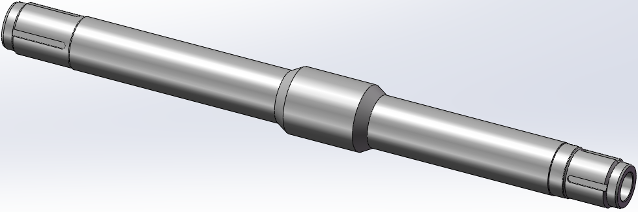
\includegraphics[width=0.7\textwidth]{figure/chapter3/part5/inner-pipe.png}
	}
	\hfill
	\subfloat[抗拉强度分析]{%
	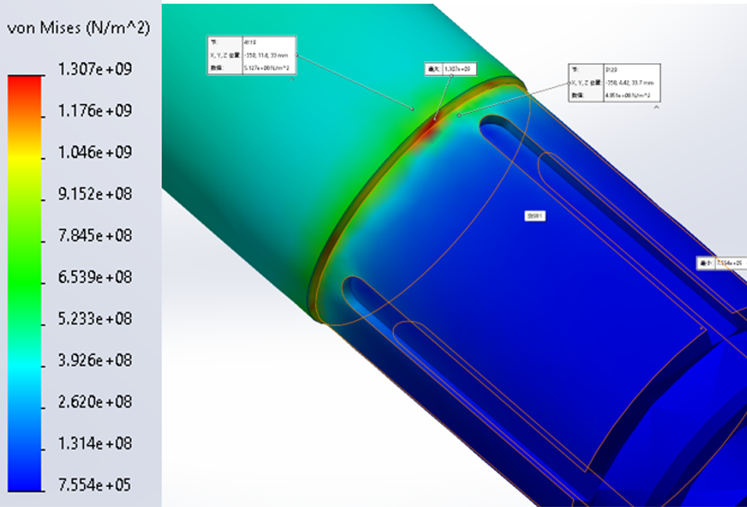
\includegraphics[width=0.4\textwidth]{figure/simulation/guadaoxinzhou-lashen.png}
	}
	\vspace{1em}
	\subfloat[抗扭强度分析]{%
	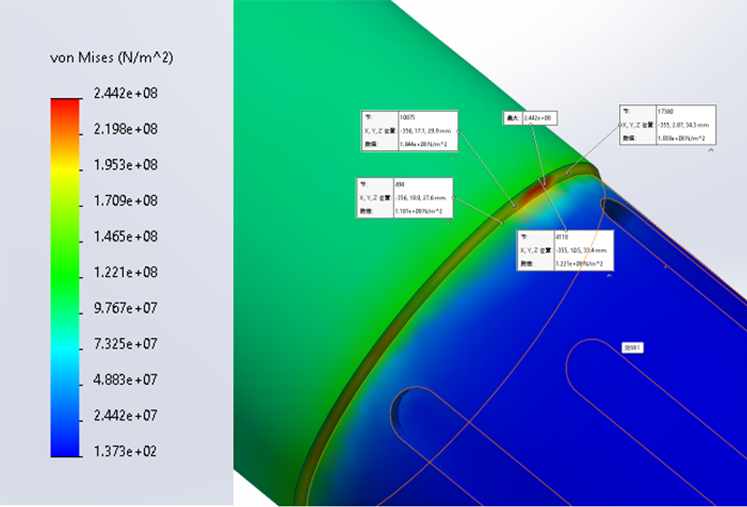
\includegraphics[width=0.3\textwidth]{figure/simulation/gaudaoxinzhou-niuju.png}
	}
	\caption{可变径刮管工具薄弱零件强度有限元分析}
	\label{fig:FEA_inner_pipe_variable}
\end{figure}


\subsection{拆装步骤}

工具入井后到达管子站进行保养前，需冲洗外表面，并准备好内六角扳手、起子、扳手等拆卸工具。

(1) 工具冲洗干净后，将上、下接头的 M16 螺钉拆卸，取出内部的防掉钢珠；取出下接头喷嘴；如下图箭头所示位置。

\begin{figure}[H]
\centering
	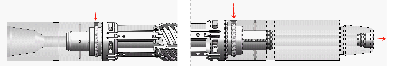
\includegraphics[width=1.\textwidth]{figure/chapter3/part5/unsetup/ball.png}
\end{figure}

(2) 拆卸上、下接头的防松螺钉后，分别反转拆卸上、下接头；如下图所示位置。

\begin{figure}[H]
\centering
	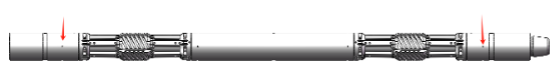
\includegraphics[width=1.\textwidth]{figure/chapter3/part5/unsetup/unsetup-satefy-screw.png}
	\vspace{1em}
	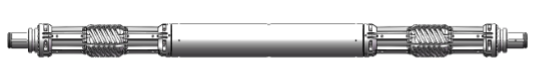
\includegraphics[width=1.\textwidth]{figure/chapter3/part5/unsetup/unsetup-two-subs.png}
\end{figure}

(3) 用起子、扳手取下连杆座、连杆、刮刀等之间的铰链销、防掉螺钉等标准件后，依次拆卸旋转连杆座、连杆、刮刀等零件；如下图所示。

\begin{figure}[H]
\centering
	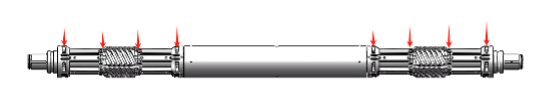
\includegraphics[width=1.\textwidth]{figure/chapter3/part5/unsetup/unsetup-fasten-parts.png}
\end{figure}

(4) 拆卸各部位的锁紧螺钉、铰链销、防掉螺钉等零件。

(5) 拆卸两头的旋转连杆座。

\begin{figure}[H]
\centering
	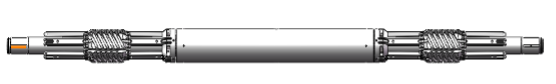
\includegraphics[width=1.\textwidth]{figure/chapter3/part5/unsetup/rotary-lever-set.png}
\end{figure}

(6) 拆卸两头的连杆、刮刀等零件。

\begin{figure}[H]
\centering
	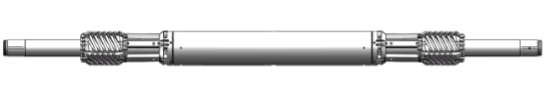
\includegraphics[width=1.\textwidth]{figure/chapter3/part5/unsetup/end-links.png}
	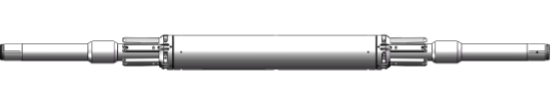
\includegraphics[width=1.\textwidth]{figure/chapter3/part5/unsetup/unsetup-scraper.png}
	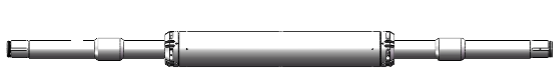
\includegraphics[width=1.\textwidth]{figure/chapter3/part5/unsetup/left-links.png}
\end{figure}

(7) 分别反转拆卸两头的芯轴，从下部取出激活球座和钢球，如下图所示。

\begin{figure}[H]
\centering
	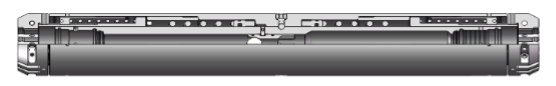
\includegraphics[width=1.\textwidth]{figure/chapter3/part5/unsetup/unsetup-inner-pipe.png}
	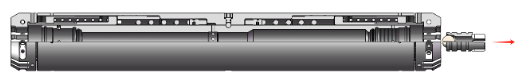
\includegraphics[width=1.\textwidth]{figure/chapter3/part5/unsetup/unsetup-ball-and-seat.png}
\end{figure}

(8) 夹紧中间外筒方向旋转复位总成，分别取出上、下两头的复位总成，然后依次对复位总成进行拆解，如下图所示。

\begin{figure}[H]
\centering
	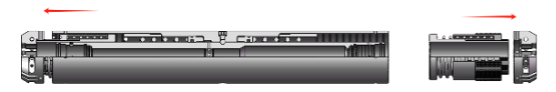
\includegraphics[width=1.\textwidth]{figure/chapter3/part5/unsetup/reseting-assembly.png}
	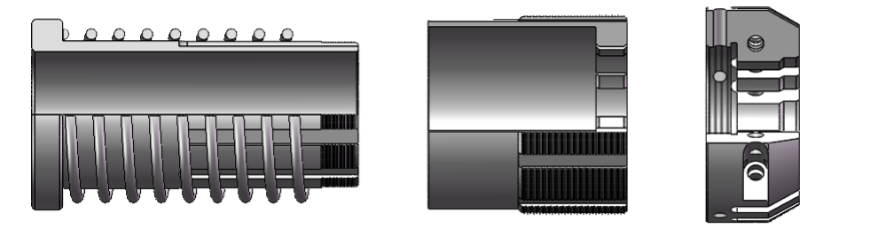
\includegraphics[width=1.\textwidth]{figure/chapter3/part5/unsetup/resetting-assembly-unsetup.png}
\end{figure}

(9) 取出中间筒体和中间芯轴的限位钢球，随后取下中间芯轴、弹簧、活塞、活塞限位套等零件；最后拆卸各零件上的密封圈，即拆卸完毕。

(10) 拆卸中间筒体和中间芯轴的钢球堵和限位钢球。

\begin{figure}[H]
\centering
	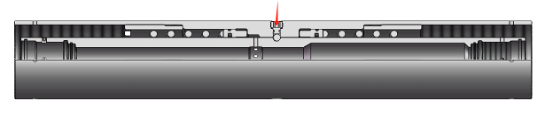
\includegraphics[width=1.\textwidth]{figure/chapter3/part5/unsetup/middle-body-inner-pipe-ball.png}
\end{figure}

(11) 拆卸中间芯轴，固定中间筒体后从任意一头抽出中间芯轴即可。

\begin{figure}[H]
\centering
	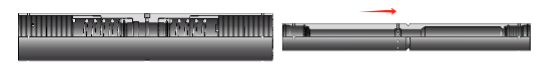
\includegraphics[width=1.\textwidth]{figure/chapter3/part5/unsetup/middle-inner-pipe-unsetup.png}
\end{figure}

(12) 按下图所示方向，分别从两头拆卸活塞、工作弹簧、活塞限位套等零件。

\begin{figure}[H]
\centering
	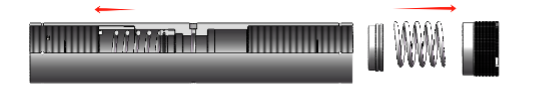
\includegraphics[width=1.\textwidth]{figure/chapter3/part5/unsetup/piston-spring-limiter.png}
\end{figure}

(13) 装配步骤与拆卸步骤相反，装配过程中需要注意不要损伤密封面、螺纹牙形等配合处，密封面和螺纹组装前要求涂抹润滑油。

工具的易损件及配件清单见表~\ref{tab:parts_list}。

\begin{table}[htbp]
    \centering
    \caption{易损件及配件清单表（按图纸BJG700000A总装图明细栏）}
    \label{tab:parts_list}
    \footnotesize % 代号较长，缩小字号以适应表格宽度
    \setlength{\tabcolsep}{4pt} % 减小列间距，避免超出正文版心
    \renewcommand{\arraystretch}{1.35} % 调整行间距，使表格不拥挤
    \begin{tabular}{clllc}
        \toprule
        \textbf{序号} & \textbf{代号} & \textbf{名称} & \textbf{材料} & \textbf{单套数量} \\
        \midrule
        1  & BJG700001A & 上接头 & 4145H & 1 \\
        2  & BJG700002A & 上活动连杆座 & 4145H & 2 \\
        3  & BJG700003A & 连杆 & 4145H & 20 \\
        4  & BJG700004A & 刮刀芯轴 & 4330V（屈服强度$1068\,\mathrm{MPa}$） & 2 \\
        5  & BJG700005A & 活动座铰链销 & 4145H & 20 \\
        6  & BJG700006A & 59BPF刮刀 & 20CrNiMo & 10 \\
        7  & BJG700007A & 刮刀铰链销 & 4145H & 20 \\
        8  & BJG700008A & 下活动连杆座 & 4145H & 2 \\
        9  & BJG700009A & 连杆座连接筒 & 4145H & 2 \\
        10 & BJG700010A & 中间调节堵 & 4145H & 2 \\
        11 & BJG700011A & 中间限位套 & 4145H & 2 \\
        12 & BJG700012A & 中间活塞 & 4145H & 2 \\
        13 & BJG700013A & 中间筒体 & 4145H & 1 \\
        14 & BJG700014A & 心轴连接筒 & 4330V（屈服强度$1068\,\mathrm{MPa}$） & 1 \\
        15 & BJG700015A & 球座 & 4145H & 1 \\
        16 & BJG700016A & 丝堵 & 316 & 2 \\
        17 & BJG700017A & 密封堵 & 316 & 2 \\
        18 & BJG700018A & 复位弹簧 & 60Si2MnA & 2 \\
        19 & BJG700019A & 工作弹簧 & 60Si2MnA & 2 \\
        20 & BJG700020A & 下接头 & 4145H & 1 \\
        21 & BJG700021A & 支撑弹片 & 50CrVA & 20 \\
        22 & BJG700022A & 弹片压块 & 4145H & 20 \\
        23 & BJG700023A & $\phi 25$ 节流喷嘴 & YG6 & 1 \\
        24 & GB/T 77-2007 & 内六角平端紧定螺钉 M10$\times$35 & 钢 12.9级 & 20 \\
        25 & GB/T 77-2007 & 内六角平端紧定螺钉 M16$\times$12 & 钢 12.9级 & 2 \\
        26 & GB/T 80-2007 & 内六角凹端紧定螺钉 M5$\times$16 & 钢 12.9级 & 40 \\
        27 & GB/T 77-2007 & 内六角平端紧定螺钉 M8$\times$8 & 钢 12.9级 & 8 \\
        28 & GB/T 79-2007 & 内六角圆柱端紧定螺钉 M10$\times$25 & 钢 12.9级 & 10 \\
        29 & GB/T 80-2007 & 内六角凹端紧定螺钉 M8$\times$10 & 钢 12.9级 & 8 \\
        30 & GB/T 80-2007 & 内六角凹端紧定螺钉 M8$\times$30 & 钢 12.9级 & 8 \\
        31 & GB/T 77-2007 & 内六角平端紧定螺钉 M8$\times$16 & 钢 12.9级 & 10 \\
        32 & GB/T 70.1-2008 & 内六角圆柱头螺钉 M6$\times$12 & 钢 12.9级 & 20 \\
        33 & GB/T 308.1-2013 & 钢球 12-G40 & G95Cr18 & 100 \\
        34 & GB/T 308.1-2013 & 钢球 30-G20 & G95Cr18 & 1 \\
        35 & NL6 & 防松垫片 & 65Mn HRC39--44 & 20 \\
        36 & 2-143 & O 形圈 $\phi 61.6\times2.62$ & FKM90 & 2 \\
        37 & 2-140 & O 形圈 $\phi 56.82\times2.62$ & FKM90 & 2 \\
        38 & 2-147 & O 形圈 $\phi 67.95\times2.62$ & FKM90 & 2 \\
        39 & 2-222 & O 形圈 $\phi 37.69\times3.53$ & FKM90 & 2 \\
        40 & 2-243 & O 形圈 $\phi 104.37\times3.53$ & FKM90 & 2 \\
        41 & 2-223 & O 形圈 $\phi 40.87\times3.53$ & FKM90 & 1 \\
        42 & 2-110 & O 形圈 $\phi 9.19\times2.62$ & FKM90 & 2 \\
        43 & ON 0800 052 00110 D & 双作用格莱圈 & FKM90+PTFE & 2 \\
        \bottomrule
    \end{tabular}
\end{table}


\subsection{操作方式}

\subsubsection{下井前准备}
\begin{itemize}
	\item 了解井况，确定套管规格和深度等基本信息；
	\item 选配适合套管规格的刮刀；
	\item 本可变径刮管器应与 7\inch 及以上其它刮管器配合使用；本工具刮刀收回外径 136\,mm、本体最大外径 139.5\,mm，在 7\inch 套管内与井壁不接触，7\inch 套管的刮管应由同趟管柱中位于本工具下方的常规 7\inch 刮管器完成；
	\item 确定刮管工艺，了解泵压和排量，并根据图~\ref{fig:pressure_decrease_with_Q_size}所示不同排量下喷嘴尺寸与压降的关系选装合适的喷嘴及剪钉。
\end{itemize}

\begin{figure}[htbp]
	\centering
	\subfloat[10L/s]{%
	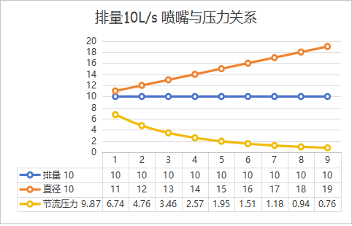
\includegraphics[width=0.4\textwidth]{figure/chapter3/part5/10LperSec.png}
	}
	%\hfill
	\subfloat[20L/s]{%
	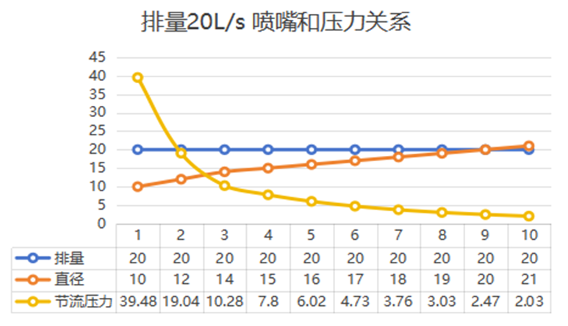
\includegraphics[width=0.4\textwidth]{figure/chapter3/part5/20LperSec.png}
	}
	\vspace{1em}
	\subfloat[30L/s]{%
	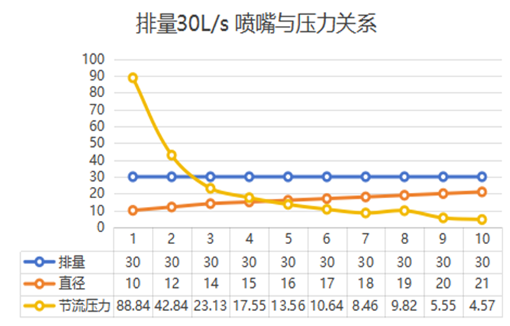
\includegraphics[width=0.4\textwidth]{figure/chapter3/part5/30LperSec.png}
	}
	\subfloat[40L/s]{%
	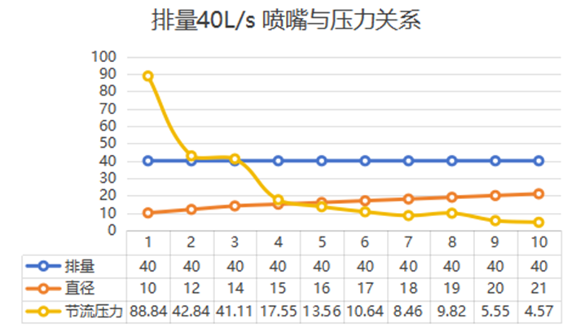
\includegraphics[width=0.4\textwidth]{figure/chapter3/part5/40LperSec.png}
	}
	\caption{喷嘴压降与排量、喷嘴尺寸之间的关系}
	\label{fig:pressure_decrease_with_Q_size}
\end{figure}

\subsubsection{作业顺序}
可变径刮管器的完整作业顺序为"先小规格套管、后 9-5/8\inch 套管；投球一次、激活不可逆"，具体步骤如下：

\begin{enumerate}[label=(\arabic*),leftmargin=2em,itemsep=2pt]
	\item \textbf{入井前检查与选配}：确认套管规格与井深；检查刮刀能否自由收回至 136\,mm、球座圆周 $4\times\phi 4.80$ 剪钉是否完好；按设计排量选装节流喷嘴（标准件为 $\phi 25$ 喷嘴 BJG700023A）；备好并登记现场投球用 $\phi 30$ 钢球（图纸明细栏"钢球 30-G20"1 件）。需注意明细栏中 100 件 $\phi 12$ 钢球（钢球 12-G40）为装配用限位钢球，不是现场投球，二者不得混用。
	\item \textbf{组配管柱}：下井前按照作业要求依次连接好管柱，刮管器前端需接与套管规格对应的扶正器；推荐管柱组合为：通井钻头 $+$ 扶正器 $+$ 7\inch 刮管器 $+$ 可变径刮管器 $+$（选装其它套管清洁工具）$+$ 上部钻柱。
	\item \textbf{地面试循环}：接上可变径刮管器后，夹紧下接头、大钳打上接头，拧紧刮管器各螺纹，井口以开泵压力 $\le 20 \pm 5\,\mathrm{MPa}$、排量 $\le 10\,\mathrm{L/s}$ 进行试循环，时间 $1 \sim 5\,\mathrm{min}$；确认循环正常、各连接无刺漏，并确认刮刀未弹出本体（仍为收回状态）。此时未投球、球座未憋压，泵压不作用于球座，刮刀不会张开。
	\item \textbf{下钻}：控制下放速度，慢慢旋转下放工具；全程保持钻井液循环畅通。本工具在 9-5/8\inch 与 7\inch 套管中均为收回通过状态，不参与刮削。
	\item \textbf{7\inch 套管段作业}：在 7\inch 套管内由下部常规 7\inch 刮管器完成刮管，并进行其它钻磨、完井、试油、测试等作业。本工具此时未激活、不参与 7\inch 段刮削；7\inch 段的全部作业必须在投球激活之前完成。
	\item \textbf{上提至 9-5/8\inch 套管井段}：当小规格套管刮管及其它作业完成后，将可变径刮管器提升至 9-5/8\inch 套管所需的井深位置，确认工具已完全脱离 7\inch 段（含尾管悬挂器、回接筒等小内径部位）后，投入 $\phi 30$ 钢球，开泵打压激活刮刀张开，启动作业。
	\item \textbf{憋压激活}：刮管器打开压力 $=$ 静液柱压力 $+$ 泵压（绝对压力），即泵压 $\ge$ 绝对压力 $-$ 静液柱压力；按\ref{kebianjingguaguan}节计算，球座剪钉剪断所需的最小泵压为 $15.5\,\mathrm{MPa}$（按塑性材料系数）$\sim 20.7\,\mathrm{MPa}$（按脆性材料系数），现场应以先达到该泵压再回落作为激活判据。
	\item \textbf{激活判定}：投入钢球后观察泵压，若泵压上升过程中突然下降，说明可变径刮管器已启动；随后停泵，按工具入井前选定的喷嘴尺寸所要求的泵压和排量稳定循环，同时通过上提、下放工具进行 9-5/8\inch 套管的刮管作业。
	\item \textbf{9-5/8\inch 套管刮管}：在稳定循环（节流工作压差 $\le 4\,\mathrm{MPa}$）条件下上提、下放工具刮削；刮管作业时观察指重表无任何显示，即下放悬重不降、上提悬重不升，表明已刮削干净。
	\item \textbf{停泵、起钻}：刮管作业完成后先停泵，使节流压差消失、刮刀由复位弹簧收回至 136\,mm，再按规定的起钻速度起出管柱；起钻过程中注意悬重与摩阻变化。
	\item \textbf{出井拆检与保养}：按拆装步骤拆开清洗，更换全部 O 形圈与失效弹簧，检查球座、剪钉孔、刮刀、铰链销及密封面，并按要求保养存放。
\end{enumerate}

\subsubsection{注意事项}
\begin{itemize}
	\item 工具与管柱的连接扣必须拧紧。
	\item 两组刮刀的螺旋升角应保持同方向。
	\item 可变径刮管器在下井过程中如遇阻，应慢慢旋转几圈后再下放。
	\item 刮管作业过程中，必须始终保持钻井液循环畅通。
	\item 工具激活为一次性、不可逆过程，图纸明细栏中不设复位球，因此不得在 7\inch 套管内投球激活，也不得在 7\inch 段作业尚未全部完成时投球。
	\item 激活后带泵循环时刮刀处于张开状态（自由张开外径 229\,mm 以上），禁止带泵循环、带压进入 7\inch 套管或任何内径小于刮刀张开外径的井段，以免顶死刮刀、损坏连杆与铰链销甚至造成卡钻；起钻通过小内径井段前应先停泵，并确认刮刀已收回。
	\item 刮刀张开后受套管内径约束贴壁，实际工作直径即 9-5/8\inch 套管内径；不得以盲目提高泵压的方式追求刮削效果，工作压差由节流喷嘴限定在 $4\,\mathrm{MPa}$ 以内，刮净以指重表判据为准。
\end{itemize}

\subsection{维护与保养}
\begin{itemize}
	\item 出井后应清洗干净，并检查各零件，如弹簧失效必须更换。各螺纹涂螺纹脂，各零件涂油，存放在阴干处。
	\item 每次作业后，都应将工具完全拆开并清洗，更换所有 O 形圈和损坏的弹簧，检查刮管器本体上的内套是否粘接牢固。用肉眼检查所有的密封面和接头丝扣是否损坏，若发现有损坏的零件都应更换，这些损坏的零件对工具的可靠性会产生不利的影响。
	\item 在拆卸、保养前，应准备好正确、有效的装配图和工具保养维护说明书及工具维护保养单。
	\item 对高温井作业以及有酸及硫化氢存在的修井作业，应提前更换相应耐腐蚀、耐高温的密封件和配件。
	\item 有关该工具使用和维护保养的其他任何问题，请与我校联系。
\end{itemize}



\section{清洁工具组合工艺}

根据不同井况需求进行清洁工具组合，减少下钻趟数，提高作业效率。9-5/8\inch 井筒深度清洁作业中，常用的管柱组合（自上而下）如下，实际作业时可根据井况要求进行调整与扩展：

（1）钻杆 $+$ 震击器 $+$ 钻杆 $+$ 9-5/8\inch 多功能过滤工具 $+$ 短钻杆 $+$ “四合一”集成式井筒清洁工具 $+$ 短钻杆 $+$ 浮阀 $+$ 钻头；

（2）钻杆 $+$ 震击器 $+$ 钻杆 $+$ 9-5/8\inch 多功能过滤工具 $+$ 短钻杆 $+$ “四合一”集成式井筒清洁工具 $+$ 循环洗井阀 $+$ 短钻杆 $+$ “三合一”集成式井筒清洁工具；

（3）钻杆 $+$ 震击器 $+$ 钻杆 $+$ 9-5/8\inch 多功能过滤工具 $+$ 短钻杆 $+$ “四合一”集成式井筒清洁工具 $+$ 循环洗井阀 $+$ 短钻杆 $+$ 可变径刮管工具。


\section{本章小结}

针对连续砂床、严重出砂井况下常规水力冲砂效率低、除砂效果差，以及套管内壁结垢、铁磁性碎屑残留、缩径与变径等井筒清洁难题，本章按照“冲—刮—刷—吸—滤—通”多功能协同的思路，完成了“三合一”脉冲式冲刮刷集成式井筒清洁工具、“四合一”通刮刷磁集成式井筒清洁工具、大容量强磁吸附工具、多功能过滤工具和可变径刮管工具共五类工具的结构设计、理论计算、仿真校核与使用维护研究，主要结论如下：

（1）“三合一”脉冲式冲刮刷集成式井筒清洁工具。

结构上由脉冲发生模块与旋转喷头模块构成，并配置毛刷刮管模块。旋转喷头模块利用两组偏心夹角喷嘴射流产生的反冲力矩驱动喷头自转，实现套管内壁 360° 无死角的周向冲洗；脉冲发生模块通过活塞—矩形弹簧机构把地面泵注的稳态液流转化为高、负压交替的低频水力脉冲波，其轴向机械振荡与径向水力冲击相叠加，可破坏压实砂床的结构、为环空砂砾补充扰动动能，抑制砂砾再沉积。
	
针对工具内部流体压力与机械部件的耦合机制，基于连续性方程与牛顿运动定律建立了包含蓄能、开启、喷射与复位四个阶段的非线性常微分方程组，形成了脉冲发生模块的瞬态动力学模型。在典型工况（$Q=50\mathrm{m^3/h}$、$K=757176\mathrm{N/m}$、侧向出水孔高度 $l_1=75\mathrm{mm}$）下，活塞最大冲程为 $88.13\mathrm{mm}$，单次工作周期为 $12.86\mathrm{ms}$，对应工作频率为 $77.76\mathrm{Hz}$。
	
参数影响规律表明：输入排量是决定脉冲特性的首要参数，在 $46\sim58\mathrm{m^3/h}$ 的设计区间内，活塞最大冲程随排量近似线性增长，正向速度峰值由 $14.5\mathrm{m/s}$ 增至 $23.1\mathrm{m/s}$，工作频率随排量提高而非线性增大；矩形弹簧刚度增大使活塞冲程阶梯式下降、单次循环时间缩短、工作频率升高；侧向出水孔高度增大则蓄能阶段延长、工作频率降低、开孔有效余量减小。设计时需在冲程与频率之间取得平衡，并保证适宜的开孔有效余量。

强度校核方面，脉冲器危险截面（螺纹应力分散槽处）的许用拉力为 $690.8\mathrm{kN}$，大于 $400\mathrm{kN}$ 的设计要求；许用扭矩为 $11.74\mathrm{kN\cdot m}$，大于 $8\mathrm{kN\cdot m}$ 的设计要求；脉冲器心轴的最大拉应力为 $630\mathrm{MPa}$，小于设计要求，最大切应力为 $994\mathrm{MPa}$，但范围极小，属应力集中引起的局部小尺度高应力，不会引发整体塑性变形。
	
冲洗效果方面，Fluent 欧拉多相流仿真表明，使用该工具后井筒内砂砾质量较无工具对照组降低了 19\%，喷嘴截面下方环空冲砂液轴向流速明显高于传统刚性钻杆，砂砾不再沉积于环空底部而富集于环空两侧，竖直截面上砂床前缘由距入口 $0.8\mathrm{m}$ 推进至压力出口，说明该工具能有效抑制砂砾在工具处的沉积并显著提升携砂与清砂效率；喷头流动仿真表明，射流冲击压力先使污染物破裂松动，随后持续的剪切应力把松动的污染物卷吸进入主流，其中低频脉动负责大块污垢的宏观剥离、高频脉动负责残留微粒的清除，因此实际应用中应根据污垢特性（硬度、厚度、黏附性）调整脉冲频谱，必要时采用复合频率策略。


（2）“四合一”通刮刷磁集成式井筒清洁工具。该工具集通井扶正、机械刮削、刷洗清扫与强磁吸附（“通、刮、刷、磁”）四项功能于一体，采用长轴式模块化布局，形成 7\inch、9-5/8\inch、13-3/8\inch 三种规格，刮刀、毛刷与磁吸模块可根据井况选装组合；刮刀采用弹簧浮动加载与可更换齿形刀片，遇顽固坚硬杂物时扭曲弹簧可压缩储能并在越障后释放，起到缓冲保护作用。校核结果表明：7\inch 规格心轴上 $2.75''\text{-}8$ Stub ACME 连接螺纹的抗拉能力为 $2851.13\mathrm{kN}$，心轴两个危险截面（内、外螺纹根部）的抗拉能力分别为 $1406.08\mathrm{kN}$ 与 $1435\mathrm{kN}$，均大于 $1000\mathrm{kN}$ 的抗拉设计指标；心轴两个危险截面的抗扭能力分别为 $31.63\mathrm{kN\cdot m}$ 与 $59.39\mathrm{kN\cdot m}$，端面键的抗扭能力为 $23.09\mathrm{kN\cdot m}$，均大于 $17\mathrm{kN\cdot m}$ 的抗扭设计指标。刮板刮削效果评价试验表明，所设计的刮板能以脆性崩碎的方式有效刮除重晶石/钡锶类硬垢，刮痕深度随弹簧压缩量的增大呈“先较快增加、后趋于饱和”的非线性响应，弹簧预紧力存在最优工作区间；工程应用中应结合套管实际内径匹配刮刀外径与弹簧预紧量，避免盲目增大预紧力，并配合循环冲洗及时排屑，以延缓刀齿堵塞、延长刮板的使用寿命。

（3）大容量强磁吸附工具。工具采用上部（侧吸、带窗保护管，适于吸附小尺度铁质颗粒）与下部（环吸、开放式，适于吸附大尺度铁质碎屑）双强磁结构组合，实现了沿沟槽方向与沿圆周方向的多方向、多尺寸磁性碎屑吸附，永磁块可单独更换、装配数量可按碎屑含量调节，吸附容量可调。经计算，7\inch、17lb/ft 套管下单根工具的吸附容量为 $28.26\mathrm{L}$，两根工具组合后的吸附容量为 $56.52\mathrm{L}$，大于 $50\mathrm{L}$ 的吸附容量设计要求；主要受力件的螺纹强度、抗拉与抗扭强度均满足设计要求：芯轴 2.85\inch-8 Stub ACME 外螺纹根部许用拉力 $1627.42\mathrm{kN}$、内螺纹根部 $2462.93\mathrm{kN}$，抗扭能力分别为 $35.98\mathrm{kN\cdot m}$ 与 $86.29\mathrm{kN\cdot m}$，均大于抗拉 $1000\mathrm{kN}$、抗扭 $18\mathrm{kN\cdot m}$ 的设计指标；下接头防退扣根部最大等效应力为 $1030\mathrm{MPa}$，略高于屈服强度，属防退扣根部几何突变引起的局部小尺度高应力，按距根部 $4\sim6\mathrm{mm}$ 处的等效应力评定满足要求，下接头端面键按 6 键同时受剪计算的许用防退扣扭矩为 $35.7\mathrm{kN\cdot m}$，亦满足指标要求。永磁材料选型方面，考虑本项目 $150^\circ\mathrm{C}$ 的温度设计指标，对比钐钴（SmCo5）与钕铁硼（N45UH）等材料的退磁曲线后，确定选用耐温性与抗退磁能力更好的钐钴材料；基于 ANSYS Maxwell 的仿真研究表明，上部结构宜采用径向充磁、下部结构宜采用周向（交叉径向）充磁，以获得均匀且最大的表面磁场分布，骨架材料应选用导磁效果好、可磁化程度高的金属合金以聚集磁感线、增大磁通（采用铝制骨架时，永磁体表面磁场由 $0.7\sim1.5\mathrm{T}$ 降至 $0.3\sim0.7\mathrm{T}$，骨架沟槽表面由 $1.2\sim3.5\mathrm{T}$ 降至 $0.2\sim0.4\mathrm{T}$）。此外，从居里温度、工作温度、外部磁场、时间、机械冲击与化学侵蚀六个方面分析了永磁体的退磁影响因素，并结合工具设计给出了磁路闭合存储、不锈钢保护套防护、磁体镀镍防腐、安装规范防划伤等防退磁措施，以及强磁工具的操作方式与维护保养要求。

（4）多功能过滤工具。完成了工具总体结构设计，以及主要受力件的螺纹强度、零件强度与抗扭强度的解析校核和有限元复核：3.625\inch-8 Stub ACME 螺纹牙剪切能力为 $1690.3\mathrm{kN}$；各受力件抗拉能力分别为提升短节 $2838.8\mathrm{kN}$、滤进接头 $2759.4\mathrm{kN}$（凹槽根部 $2184.4\mathrm{kN}$）、滤出接头 $2859.0\mathrm{kN}$（凹槽根部 $1974.9\mathrm{kN}$）、下接头 $2838.8\mathrm{kN}$，均大于 $1000\mathrm{kN}$ 的设计指标；抗扭能力分别为提升短节 $65.6\mathrm{kN\cdot m}$、滤进接头 $76.4\mathrm{kN\cdot m}$、滤出接头 $78.5\mathrm{kN\cdot m}$、下接头 $135.6\mathrm{kN\cdot m}$，均大于 $18\mathrm{kN\cdot m}$ 的合同指标，其中以提升短节内螺纹根部的 $65.6\mathrm{kN\cdot m}$ 为最小，仍大于技术参数表所列的许用抗扭强度 $39\mathrm{kN\cdot m}$；针对工具两端与管柱连接的 NC38 接头（API Spec 7-2），补充了抗拉、抗扭与螺纹牙剪切校核：其过渡段圆环截面（$\phi 95.25/\phi 44.45$）的抗拉能力为 $3454\mathrm{kN}$、抗扭能力为 $99.2\mathrm{kN\cdot m}$，螺纹牙剪切能力为 $2764.1\mathrm{kN}$，均满足设计要求；有限元复核表明滤进、滤出接头变径处的峰值应力范围极小，以距变径台阶根部 $4\sim6\mathrm{mm}$ 处的等效应力作为评定值，对应屈服强度的安全系数均大于 $1.5$。过滤容积计算值为 $18.0\mathrm{L}$（过滤套筒全长范围内的几何容积），满足设计要求；同时给出了以清理盖板为核心的清理操作方式与拆洗维护要求。针对多功能过滤工具的流动与堵塞风险，补充了以下定量论证：最小流通面积由过滤内筒内孔控制，7\inch 工具（GLGJ70000A）为 $\phi 35.05\mathrm{mm}$ 对应的 $965\mathrm{mm}^{2}$（$1.50\mathrm{in}^{2}$）、9-5/8\inch 工具（GLGJ98500A）为 $\phi 68.28\mathrm{mm}$ 对应的 $3662\mathrm{mm}^{2}$（$5.68\mathrm{in}^{2}$），过滤面（开孔或绕丝缝隙）总面积为最小流通面积的 $41\sim76$ 倍、碎屑腔环空为 $0.88\sim2.78$ 倍，工具内部不存在比内孔更小的节流截面；按达西--魏斯巴赫公式计算，在 $5\sim20\mathrm{L/s}$ 排量下 7\inch 工具的内部附加压降为 $0.05\sim1.05\mathrm{MPa}$（$10\mathrm{L/s}$ 时为 $0.19\sim0.27\mathrm{MPa}$，约占泵压的 $3\%$）、9-5/8\inch 工具为 $0.003\sim0.044\mathrm{MPa}$，且 $96\%$ 以上由内孔沿程损失贡献，过滤面与碎屑腔本身的压降可忽略；过滤面积分别为 $0.935\mathrm{m}^{2}$（7\inch 加长版）、$0.700\mathrm{m}^{2}$（7\inch 标准版）和 $0.703\mathrm{m}^{2}$（9-5/8\inch），碎屑有效容纳量分别为 $9.21\mathrm{L}$、$6.90\mathrm{L}$ 和 $5.86\mathrm{L}$；碎屑充填率在 $60\%$ 以内时对循环无影响，超过 $70\%$ 后碎屑腔余隙降至 $3.7\mathrm{mm}$ 以下、附加压降随充填率非线性上升（$70\%\sim90\%$ 区间由 $0.57\mathrm{MPa}$ 增至 $22.5\mathrm{MPa}$），故以充填率 $60\%$ 为现场预警线、$70\%$ 为起钻清理控制线；由于碎屑腔与内孔流道相互独立并设有扶正套筒开关，过滤容量达到上限不会造成循环通道的完全封堵，工具具有“堵而不死”的失效安全特性。此外，通过计算指出技术参数表中 7\inch 加长版的碎屑存储量 $15.85\mathrm{L}$ 与过滤外筒实际穿孔长度（$3906.9\mathrm{mm}$）不一致，且现有两套规格的碎屑存储量均小于合同指标 $30\mathrm{L}$，建议统一“几何容积/有效容纳量”口径并进一步加长过滤段或采用双工具串接予以满足。

（5）可变径刮管工具。完成了主要受力件的螺纹强度、零件抗拉与抗扭强度校核以及刮刀芯轴、芯轴连接筒的有限元仿真校核（刮刀芯轴受拉的最大等效应力为 $1307\mathrm{MPa}$，为变径凸台处的局部峰值，按距变径处评定值 $485.9\mathrm{MPa}$ 校核满足要求；受扭的最大等效应力为 $244.2\mathrm{MPa}$，同样满足要求；芯轴连接筒按图纸内螺纹小径 $\phi 62.20$ 复核的抗拉能力为 $1414.72\mathrm{kN}$，大于 $1000\mathrm{kN}$），并计算了工具激活与节流的关键参数：球座圆周均布 4 个 $\phi 4.80$ 剪钉（图纸BJG700015A），按塑性材料系数 $0.6[\sigma]$ 计算的剪断力为 $19534.4\mathrm{N}$，按球座锥面承压直径 $\phi 40.08$ 计算的最小激活泵压为 $15.48\mathrm{MPa}$（若按脆性材料系数 $0.8[\sigma]$ 则分别为 $26045.9\mathrm{N}$ 与 $20.65\mathrm{MPa}$），节流喷嘴的最小直径为 $25.06\mathrm{mm}$（对应节流工作压差不超过 $4\mathrm{MPa}$，实取图纸标准件 $\phi 25$ 喷嘴BJG700023A），连杆销按图纸材料 4145H 及 20 个销、40 个剪切面计算所需最小直径为 $8.35\mathrm{mm}$，实取图纸 $\phi 10$ 铰链销，剪应力 $318.3\mathrm{MPa}$ 小于许用值 $456\mathrm{MPa}$。工具的规格口径与技术定位也已明确：本工具用于通过 7\inch 套管后刮削 9-5/8\inch 套管内壁，刮刀收回外径 136\,mm（本体最大外径 139.5\,mm）以保证通过 7\inch 套管，投球激活后刮刀自由张开外径 229\,mm 以上、实际受 9-5/8\inch 套管内径约束贴壁；投球前工具处于收回待命状态（球座由 4 个剪钉定位于上位，活塞腔与水眼流道被隔断，刮刀由复位弹簧保持收回），投球憋压剪断剪钉、球座下移后建立活塞腔与流道，由节流压差经工作活塞—工作弹簧—连杆机构将轴向位移转换为刮刀的径向张开，停泵后由复位弹簧收回；工具激活为一次性、不可逆过程，故 7\inch 套管段刮管及该段其它作业必须在投球之前完成，7\inch 段刮管由同趟管柱下部配套的常规 7\inch 刮管器承担，二者组合实现"一趟钻完成 7\inch 与 9-5/8\inch 套管刮管"。此外给出了拆装步骤、下井前准备、以"先小后大、投球一次、先停泵后起钻"为原则的完整作业顺序与注意事项（如以投球后泵压先升后降判断工具启动，以指重表无显示作为刮削干净的判据，禁止在 7\inch 套管内投球激活、禁止激活后带泵进入内径小于刮刀张开外径的井段），以及维护保养规程。

（6）五类工具的配套使用。三合一工具集脉冲发生、旋转喷头与毛刷刮管模块于一体，适用于冲砂洗井及套管内壁清洁；四合一工具兼具通井扶正、刮削、刷洗与磁吸功能；大容量强磁吸附工具、多功能过滤工具与可变径刮管工具既可单独使用，也可与 ZKG 模块化多合一套管清洁工具配套组合使用，从而在同一趟作业中完成通井、刮削、刷洗、铁磁性碎屑吸附与碎屑过滤收集等多项功能，减少起下钻次数。各类工具主要受力件的应力、抗拉与抗扭能力，以及吸附容量、过滤容积等功能指标，均通过理论计算或仿真校核并满足设计要求，且均配套了拆装、操作与维护保养规程，形成了“结构设计—理论计算—仿真校核—使用维护”的完整设计链条。

综上，本章所设计的五类井筒清洁工具在功能上覆盖了砂床破坏、机械刮削、刷洗清扫、强磁吸附、碎屑过滤与变径通井等井筒清洁需求，在强度与功能指标上均通过了计算与仿真校核，为下一步的室内性能试验与现场应用验证奠定了基础。
